This section uses ANSYS Mechanical FEA software \cite{ANSYS} to validate analytical findings from previous sections. Please note that all results presented in the foregoing section utilizes USC units however, important results will be converted to their respective SI units. The overall ANSYS geometry is first presented followed by a series of FEA runs which are summarized below (see Table~\ref{table:4_runs}).

\begin{table}[H]
  \centering
  \caption{Labeling of FEA runs.}
    \begin{tabular}{cll}
    \textbf{Run } & \textbf{Focus} & \textbf{Description}\\
    \hline
    1A    & Drum Stress & Fixed ends, uniform $p$\\
    1B    & Drum Stress & Simply supported ends, uniform $p$ \\
    2A    & Drum Stress & Fixed ends, Capstan $p, z=24.5$, various $\mu$ \\
    2B    & Drum Stress & Simply supported ends, Capstan $p, z=24.5$, various $\mu$ \\
    2C    & Drum Stress & Fixed ends, Capstan $p, z=0$, various $\mu$ \\
    2D    & Drum Stress & Simply supported ends, Capstan $p, z=0$, various $\mu$ \\
    3     & Drum Buckling & Simply supported ends, uniform $p$ \\
    4     & Flange Stress & Fixed ends, uniform $p$ \\
    \end{tabular}%
  \label{table:4_runs}%
\end{table}%


\section{Model}

Both $D$ and $L$ parameters from Table~\ref{table:prelim_params} are used to model the drum barrel's geometry. The coordinate system adopted in the foregoing analysis is shown below in Figure~\ref{fig:4_geom}. 

\begin{figure}[H]
	\centering
	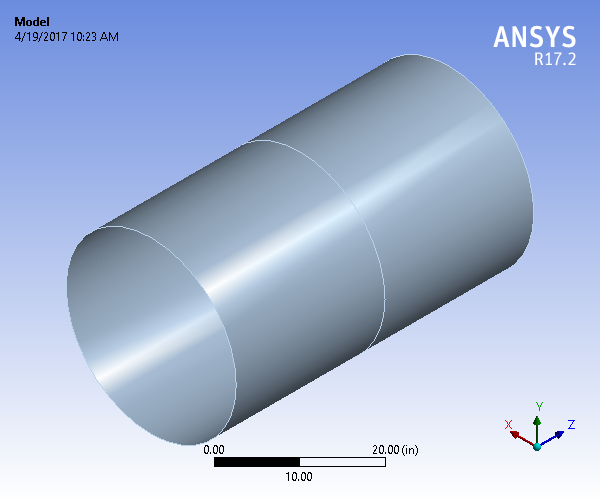
\includegraphics[scale=0.5]{4_geom}
	\caption{Geometry and coordinate system overview.}
	\label{fig:4_geom}
\end{figure}

This model utilizes a thin cylindrical surface with inwards parameterized thickness to save computational time. A series of parametric studies will be performed determine how maximum stresses vary with $t$. Note that flanges are not shown in this model as they will be added in the final run.\\

The thin surface also allows for a simple initial ANSYS generated coarse mesh (see Figure~\ref{fig:4_mesh}).

\begin{figure}[H]
	\centering
	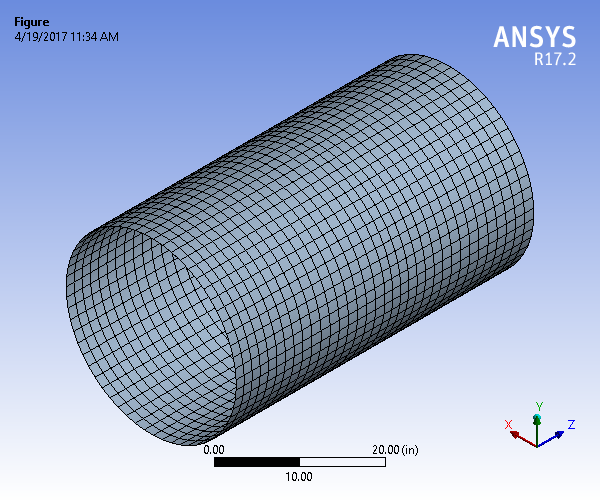
\includegraphics[scale=0.5]{4_mesh}
	\caption{Initial model coarse mesh.}
	\label{fig:4_mesh}
\end{figure}

Numerical accuracy of results will be assured by performing mesh refinement when possible in all foregoing simulations.

\section{Run 1: Uniform Pressure}
\label{section:4_R1}

The first FEA run will explore the simply uniformly loaded drum with both fixed and free ends. 

\subsection{Boundary Conditions}
\label{subsection:R1BC}

An initial simulation will be performed with fixed ends (BC as per Equation~\ref{eq:2_fixedBC}) and $t=0.500\Unit{in}$. Figure~\ref{fig:4_R1_p} shows the uniform external pressure of $1376 \Unit{psi}$ or $9.484 \Unit{MPa}$ as per \ref{eq:2_preq}.
\begin{figure}[H]
	\centering
	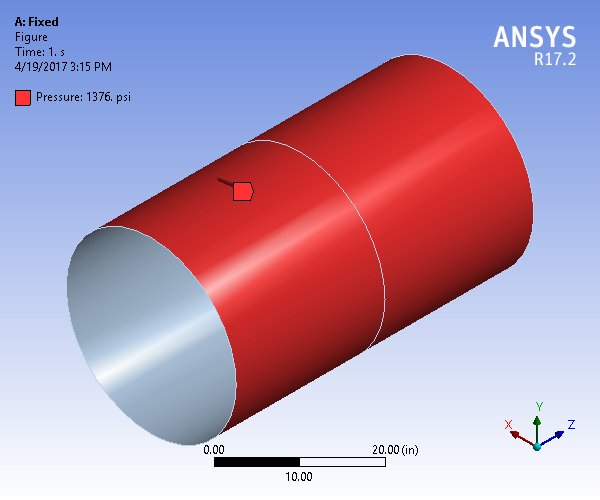
\includegraphics[scale=0.5]{4_R1_p}
	\caption{Uniform external pressure on model.}
	\label{fig:4_R1_p}
\end{figure}

\subsection{Results}

A mesh refinement is completed and yields the equivalent maximum stress results in Figure~\ref{fig:4_R1_stress} below. Note results are shown for $t=0.500\Unit{in}$.

\begin{figure}[H]
	\centering
	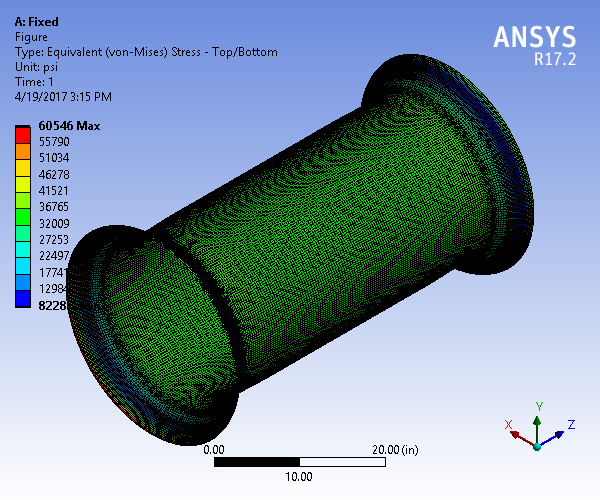
\includegraphics[scale=0.5]{4_R1_stress}
	\caption{Maximum equivalent stress results for Run 1.}
	\label{fig:4_R1_stress}
\end{figure}

It is apparent from the above figure that the fixed ends are carrying most of load. In hopes of better understanding how this uniform pressure results in stress, a parametric study will is performed by varying the drum thickness $t$ for a cylinder with both fixed and simply supported ends.


\subsection{Parametric Study}

A parametric study is perforned with a range of $t \in [0.500, 1.750]$ for both fixed and simply supported ends. The results from this simulation are shown below in Figure~\ref{fig:4_R1_sweep} \cite{EXCEL}. The allowable stress limit of $23,333 \Unit{psi}$ (Equation~\ref{eq:2_sigall}) is also shown for reference.

\begin{figure}[H]
	\centering
	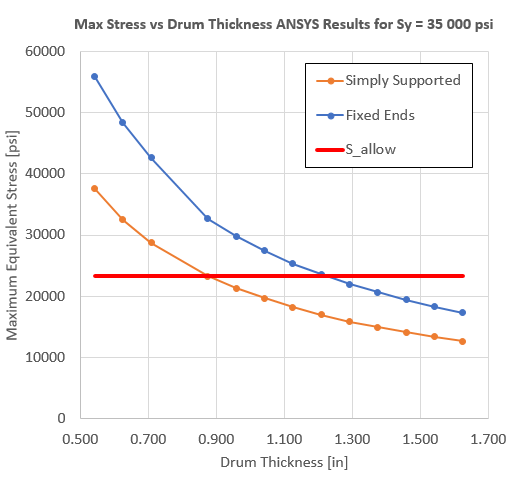
\includegraphics[scale=0.75]{4_R1_sweep}
	\caption{Results the parametric sweep for Run 1.}
	\label{fig:4_R1_sweep}
\end{figure}

From the above plot, thicknesses of $1.250 \Unit{in}$ and $0.875\Unit{in}$ are required for a uniformly loaded cylinder with fixed (Run 1A) and simply supported ends (Run 1B) respectively. These results are relatively close to their analytical counterparts. Several sources of error could be a reason for the discrepancies , those of which will be discussed in Section~\ref{subsection:5_numerr}.

\section{Run 2: Capstan Pressure}
\label{section:4_R2}
The second run elaborates on the results determined from Run 1. The aim of Run 2 is to determine how the decaying Capstan pressures translates to stress. This pressure profile represents a more realistic loading scenario.

\subsection{Boundary Conditions}

Initial results are shown for simply supported supported ends (i.e. BC as per Equation~\ref{eq:2_endBC} ) and a thickness of $0.500$ in.\\

The variable Capstan pressure is shown applied to the external surface of the cylinder in Figure~\ref{fig:4_R2_pvar}. This pressure profile is also shown in Figure~\ref{fig:4_R2_pvarplot} as per the results in Section~\ref{subsection:alt}. Note again that the pressure profile is shown for $\mu=0.05$, the worst case scenario. It is also applied beginning at the center of the drum or $z=24.5$.

\begin{figure}[H]
	\centering
	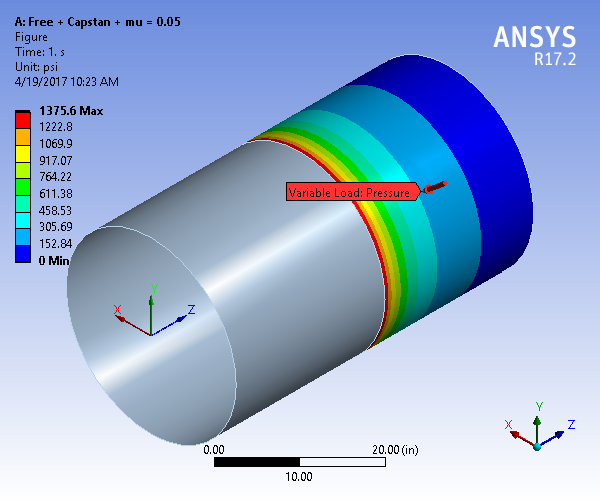
\includegraphics[scale=0.5]{4_R2_pvar}
	\caption{Variable Capstan pressure for $\mu=0.05$.}
	\label{fig:4_R2_pvar}
\end{figure}
\begin{figure}[H]
	\centering
	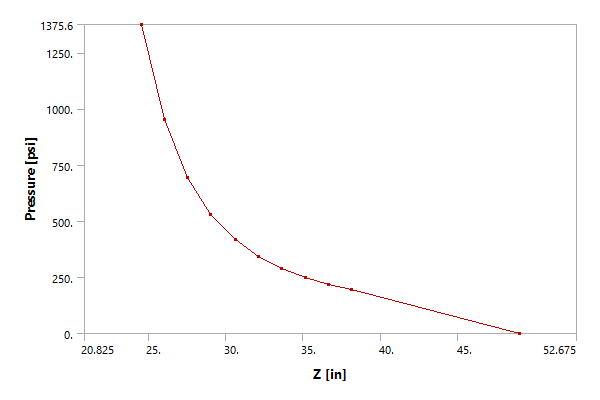
\includegraphics[scale=0.6]{4_R2_pvarplot}
	\caption{Variable Capstan pressure $p(z)$.}
	\label{fig:4_R2_pvarplot}
\end{figure}

\subsection{Results}

The maximum stress results are shown in Figure~\ref{fig:4_R2_stress_mu05} below for Run 2.

\begin{figure}[H]
	\centering
	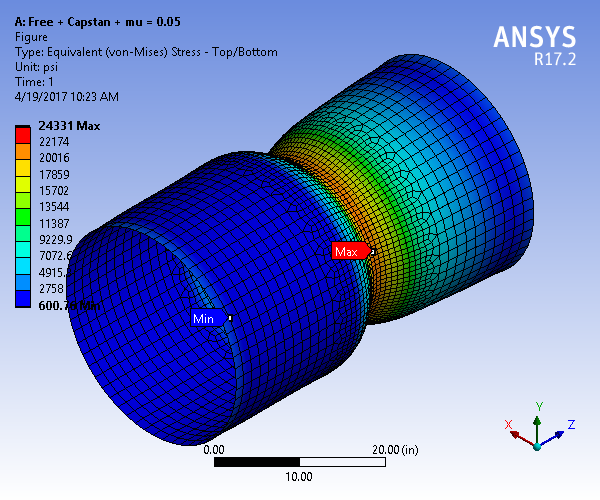
\includegraphics[scale=0.5]{4_R2_stress_mu05}
	\caption{Maximum equivalent stress results for Run 2.}
	\label{fig:4_R2_stress_mu05}
\end{figure}

Unlike the results from Run 1, it appears as though the maximum stress occurs after slightly after the location where pressure is maximum. The maximum stress is also much lower. This behavior is next explored.

\subsection{Parametric Study}

With a range of $t\in [0.15, 1.05]$, and pressure profiles for $\mu =0.05, 0.50$, maximum stress is calculated for a cylinder with both fixed and simply supported ends. The sweep results are shown below in Figure~\ref{fig:4_R2_sweep} \cite{EXCEL}.  The allowable stress limit is also shown.

\begin{figure}[H]
	\centering
	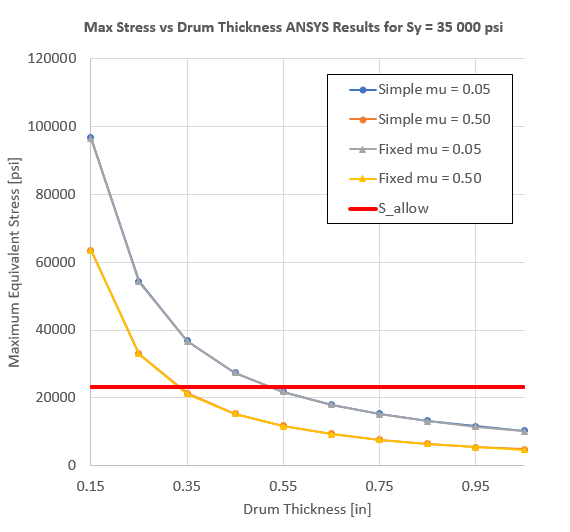
\includegraphics[]{4_R2_sweep_FE_SSE}
	\caption{Results of parametric study for FEA Run 2A-B.}
	\label{fig:4_R2_sweep}
\end{figure}

The main observation from the above sweep summary is that for a Capstan pressure profile beginning at the center of the drum ($z=24.5$) regardless of the end conditions. This observation can be validated through thin shell theory (i.e $\beta x \geq 6$) which dictates that internal ladings disappear once a certain distance is reached away from the location of the load application.\\

From the above plot, it appears as though a thickness of $t \geq 0.55 \Unit{in}$ would appear to be sufficient for both fixed (Run 2A) and simply supported ends (Run 2B).\\

To investigate the effects of the end conditions, the Capstan pressure was applied from $0 \leq z \leq 24.5$ (see Figure~\ref{fig:4_R2_BC_c}). The results for $t=0.500$ and $\mu=0.05$ with simply supported ends is shown in Figure~\ref{fig:4_R2_stress_c} for reference.
\begin{figure}[H]
	\centering
	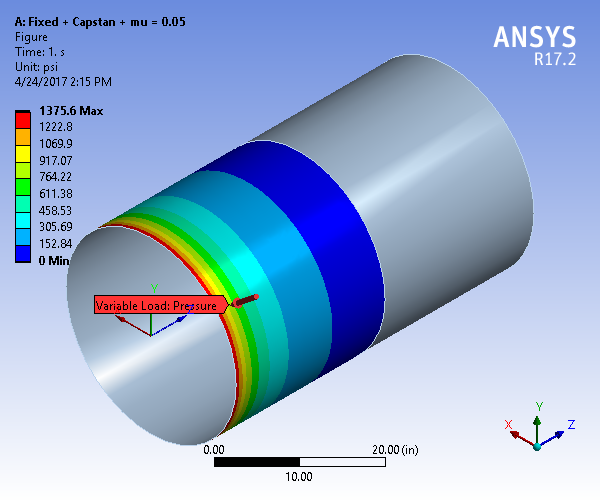
\includegraphics[scale=0.5]{4_R2_BC_c}
	\caption{Variable Capstan pressure.}
	\label{fig:4_R2_BC_c}
\end{figure}

\begin{figure}[H]
	\centering
	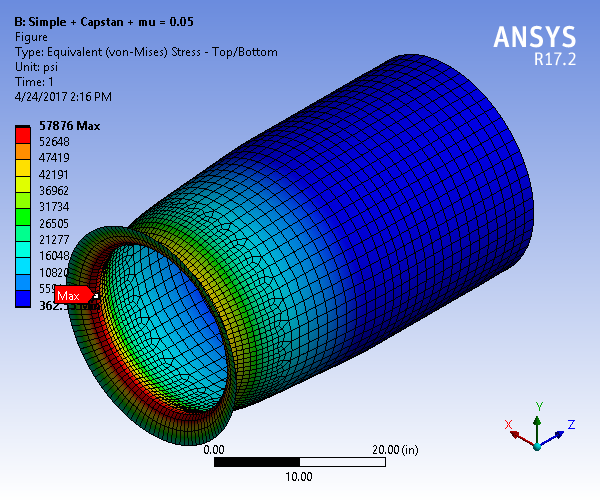
\includegraphics[scale=0.5]{4_R2_stress_c}
	\caption{Total stress results.}
	\label{fig:4_R2_stress_c}
\end{figure}

From this, a similar sweep was performed with the same aforementioned range Figure~\ref{fig:4_R2_sweep2}. With a Capstan pressure profile load applied from $0 \leq z \leq 24.5$ with $\mu=0.05$, the sweep was performed to determine the effects of the end conditions.

\begin{figure}[H]
	\centering
	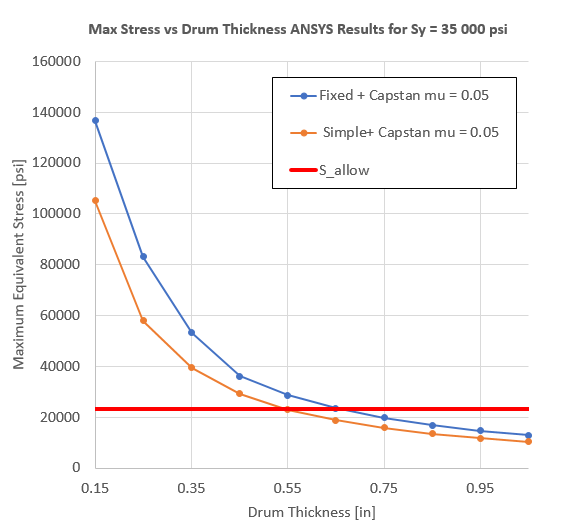
\includegraphics[]{4_R2_sweep_c}
	\caption{Results of parametric study for FEA Run 2C-D.}
	\label{fig:4_R2_sweep2}
\end{figure}

Moving the initial location of the pressure load application from $z=24.5$ to $z=0$ yields required thicknesses of $0.650$ and $0.550$ in for fixed and simply supported ends, respectively.

\section{Run 3: Eigenvalue Buckling}
\label{section:4_R3}

Buckling mode shapes do not represent actual displacements but help you to visualize how a part or an assembly deforms when buckling. \cite{ANSYS}. \\

Load factors $\lambda$ highly dependent on pre-stressed state, either linear on non linear.\\

In this case linear buckling is utilized for its simplicity. Must have coupled static structural analysis (see Figure~\ref{fig:4_R3_wb}.

\begin{figure}[H]
	\centering
	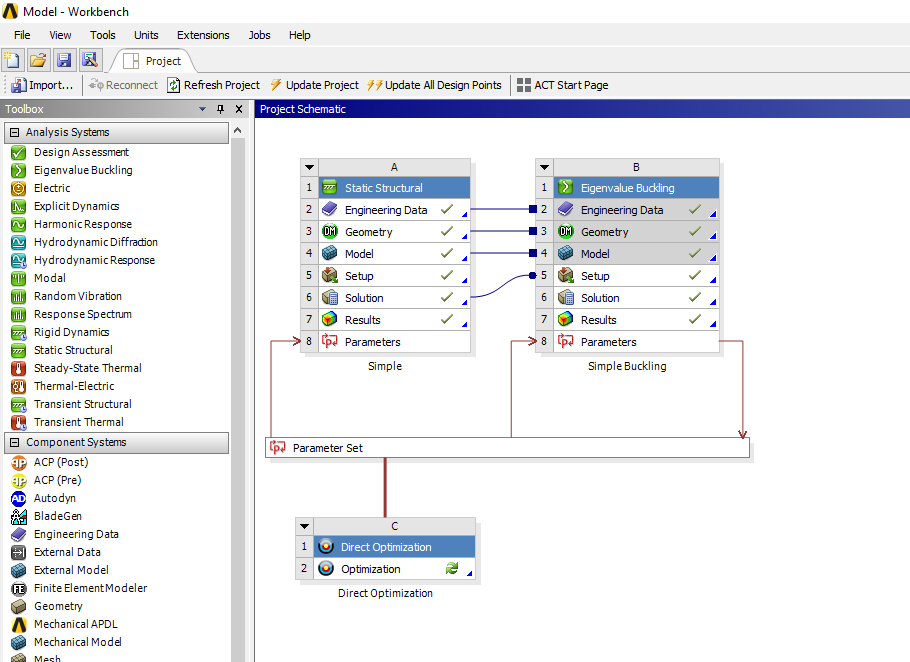
\includegraphics[scale=0.5]{4_R3_wb}
	\caption{Workbench project schematic.}
	\label{fig:4_R3_wb}
\end{figure}

ANSYS takes in the pre-stressed state and returns load factors $\lambda$ which are defined as follows in Equation~\ref{eq:4_loadfactor}.
\begin{equation}
	\label{eq:4_loadfactor}
	p' = \lambda \ p_0
\end{equation}

For this reason, a unit load pressure of $p_0 = 1\ psi$ will be applied. The boundary conditions will follow those of Section~\ref{subsection:R1BC}.

\subsection{Boundary Conditions}

Boundary conditions of coupled static structural analysis. Ends simply supported (Equation~\ref{eq:2_endBC}) and a unit pressure load applied to external surface (see Figure~\ref{fig:4_R3_BC}). Furthermore, for comparison of critical buckling calculations in Section~\ref{section:3_buckle}, a thickness of $t=0.418\Unit{in}$ was modeled. 

\begin{figure}[H]
	\centering
	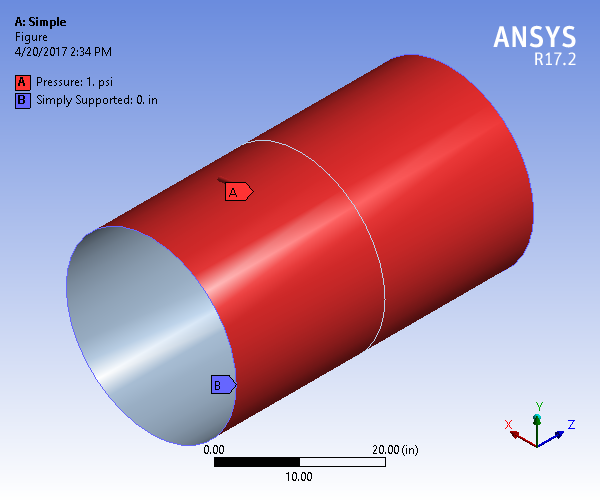
\includegraphics[scale=0.5]{4_R3_BC}
	\caption{Boundary conditions for Eigenvalue Buckling analysis.}
	\label{fig:4_R3_BC}
\end{figure}

\subsection{Results}

Unfortunately, ANSYS is unable to perform a mesh refinement study for a coupled static structural and eigenvalue buckling analysis hence, a much finer initial mesh than that shown in Figure~\ref{fig:4_mesh} was used to assure reasonably accurate results on the first iteration.\\

Results are shown below for the first eigenvalue or mode $\psi = 1$ below in Figure~\ref{fig:4_R3_mode1}.
\begin{figure}[H]
	\centering
	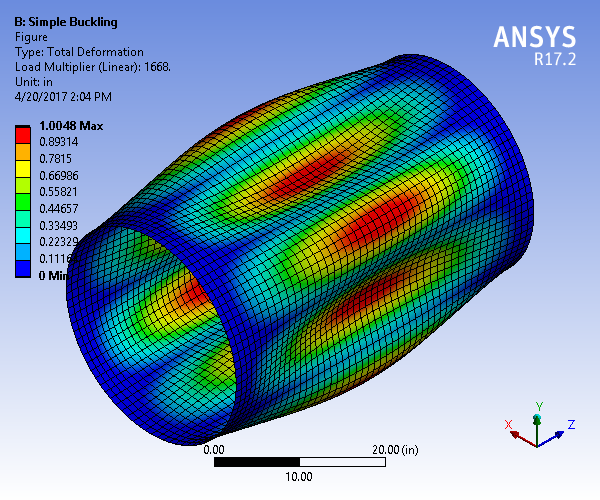
\includegraphics[scale=0.5]{4_R3_mode1}
	\caption{Total deformation results for mode $\psi = 1$.}
	\label{fig:4_R3_mode1}
\end{figure}

From above, it can be seen that a load factor of $\lambda = 1668$ was calculated for $t= 0.418\Unit{in}$. This value is within about $21.2\%$ of the expected analytical results.

\subsection{Parametric Study}

For $t\in [0.05, 1.05]$, a parametric study was performed. Results for the first, fifth and tenth mode (i.e. $\psi = 1, 5, 10$) are plotted against the thickness range of interest in Figure~\ref{fig:4_R3_modesweep} below, as per \cite{PYTHON} script in Appendix~\ref{appendix:a4}. The required critical pressure of $p =1376\Unit{psi}$ is also shown for reference.

\begin{figure}[H]
	\centering
	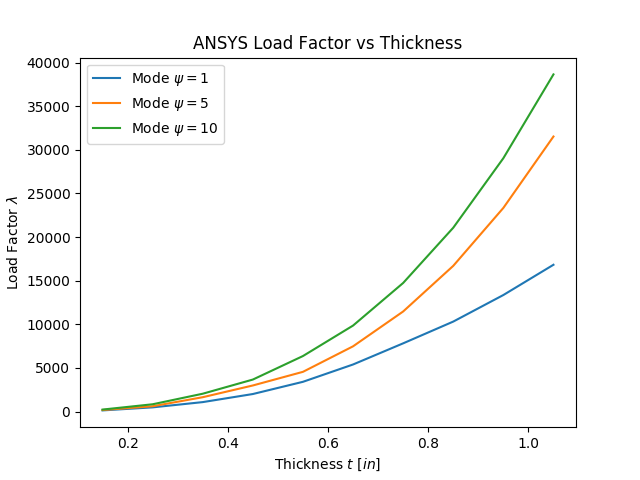
\includegraphics[scale=0.75]{4_R3_modesweep}
	\caption{Parametric sweep results for various $t, \psi$.}
	\label{fig:4_R3_modesweep}
\end{figure}

\begin{figure}[H]
	\centering
	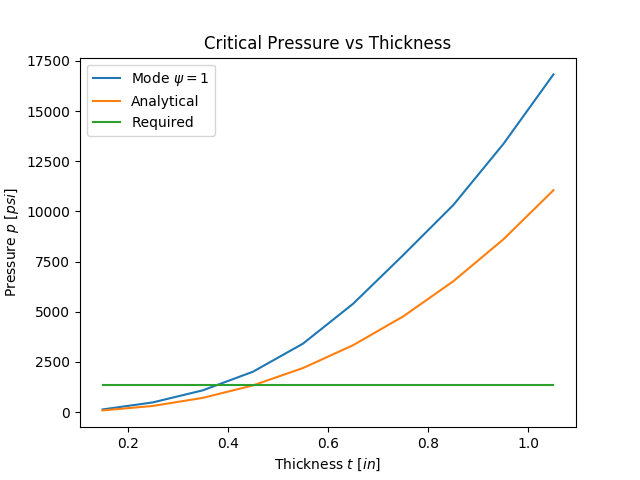
\includegraphics[scale=0.75]{4_R3_comp}
	\caption{Comparison of analytical and FEA results.}
	\label{fig:4_R3_comp}
\end{figure}


The main conclusion which can be drawn for the above results confirms those from Section~\ref{section:3_buckle} that buckling will not be the primary failure mode due to the smaller thicknesses required to attain a critical pressure of $p'$ as calculated in Equation~\ref{eq:2_preq}.

\section{Run 4: Flanges}
\label{section:4_R4}
\subsection{Model}

In hopes of finding a reasonable estimate for sizing the drum assembly's flanges, a final FEA run is completed. Figure~\ref{fig:4_R4_mesh} below shows the mesh for the modeled assembly. Note that the flanges are also modeled as thin surfaces. Drum barrel has thickness of 0.625 in which will be held constant in this section.
\begin{figure}[H]
	\centering
	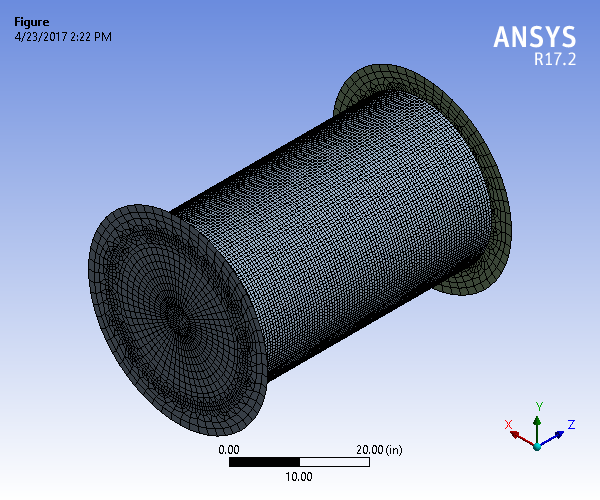
\includegraphics[scale=0.5]{4_R4_mesh}
	\caption{Drum assembly mesh.}
	\label{fig:4_R4_mesh}
\end{figure}

\subsection{Boundary Conditions}

Figure~\ref{fig:4_R4_BC} shows uniform external pressure of $1376 \Unit{psi}$ and fixed circular region on flange face of 5 in.
\begin{figure}[H]
	\centering
	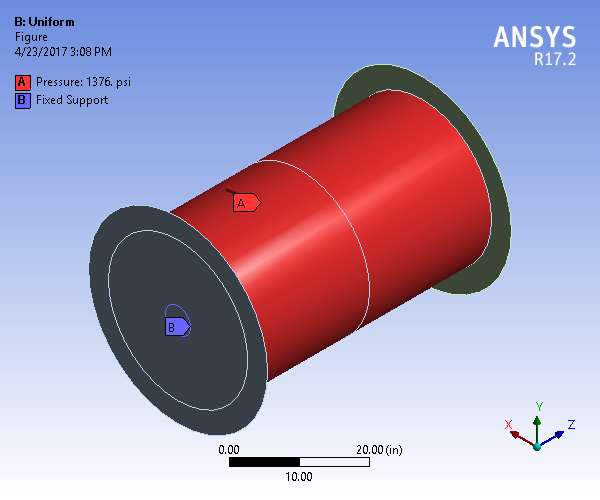
\includegraphics[scale=0.5]{4_R4_BC}
	\caption{Uniform pressure and fixed flange region.}
	\label{fig:4_R4_BC}
\end{figure}


\subsection{Results}

Figure~\ref{fig:4_R4_res2} Figure~\ref{fig:4_R4_res1}. Note results shown for flanges of thickness 0.125 in.

\begin{figure}[H]
	\centering
	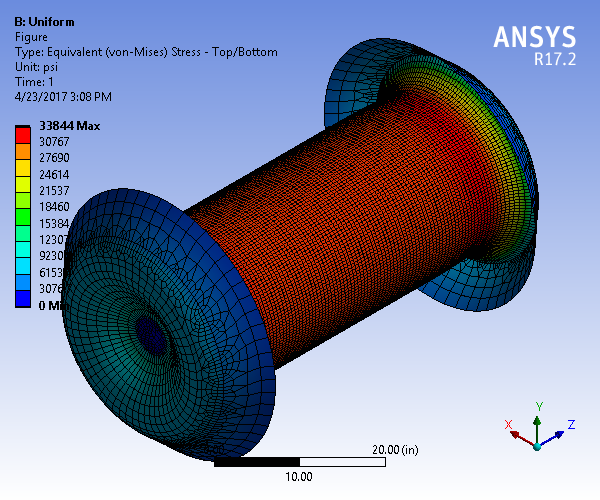
\includegraphics[scale=0.5]{4_R4_res2}
	\caption{Drum assembly stress results.}
	\label{fig:4_R4_res2}
\end{figure}
\begin{figure}[H]
	\centering
	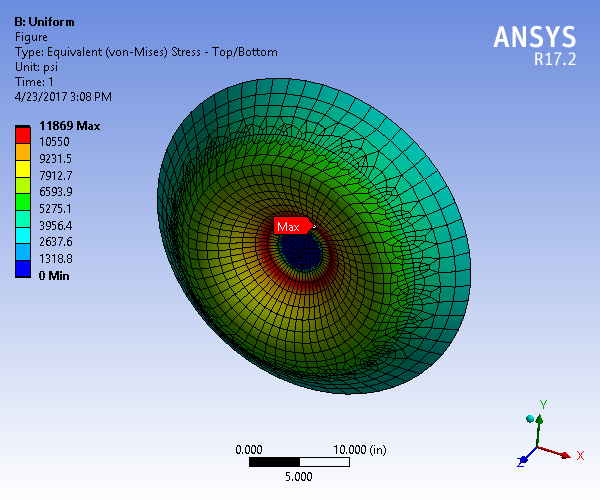
\includegraphics[scale=0.5]{4_R4_res1}
	\caption{Flange stress results for $t=0.125 \Unit{in}$.}
	\label{fig:4_R4_res1}
\end{figure}

Comments, lots of deformation.\\

\subsection{Parametric Study}

A parametric study was ran with $t \in [0.0625, 1.00]$. This sweep results are shown below in Figure~\ref{fig:4_R4_sweep} \cite{EXCEL}. The allowable stress limit of Equation~\ref{eq:2_sigall} of $23,333 \Unit{psi}$ is also shown for reference.

\begin{figure}[H]
	\centering
	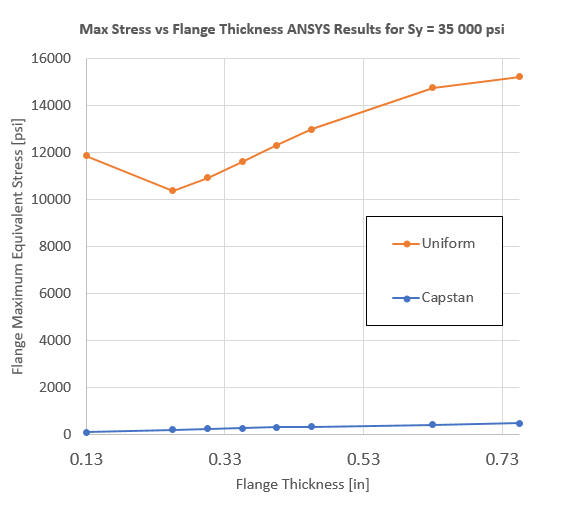
\includegraphics[]{4_R4_sweep}
	\caption{Results of parametric study for FEA Run 4.}
	\label{fig:4_R4_sweep}
\end{figure}

Upon completing this highly simplified simulation, it would appear that a thickness of $t\approx 0.25 \Unit{in}$ is the optimal candidate for the thickness of the flanges, given that a thin circular end of 5 in is held fixed. The reason for the increase in flange stress with thickness could be a result of the effects of the fixed end.

